\documentclass[12pt,a4paper]{article}

\usepackage[utf8]{inputenc}
\usepackage[T1]{fontenc}
\usepackage[spanish]{babel}
\usepackage{geometry}
\usepackage{amsmath}
\usepackage{booktabs}
\usepackage{array}
\usepackage{longtable}
\usepackage{multirow}
\usepackage[table]{xcolor}
\usepackage{graphicx}
\usepackage{float}
\usepackage{caption}
\usepackage{parskip}
\usepackage{fancyhdr}
\usepackage{titlesec}
\usepackage{hyperref}
\usepackage{listings}

\geometry{margin=2.5cm}

\definecolor{projectblue}{RGB}{18,63,106}
\definecolor{lightgray}{RGB}{245,245,245}
\definecolor{midgray}{RGB}{200,200,200}

\lstdefinestyle{evidence}{
  basicstyle=\ttfamily\small,
  backgroundcolor=\color{lightgray},
  frame=single,
  breaklines=true,
  columns=fullflexible,
  keepspaces=true,
  showstringspaces=false
}

\titleformat{\section}{\large\bfseries\color{projectblue}}{}{0em}{}[\color{projectblue}\titlerule]
\titleformat{\subsection}{\normalsize\bfseries\color{projectblue}}{}{0em}{}

\pagestyle{fancy}
\fancyhf{}
\fancyhead[L]{\small\color{projectblue}Administraci\'on de Bases de Datos}
\fancyhead[R]{\small\color{projectblue}Semana 4 --- An\'alisis Geoespacial y EDA}
\fancyfoot[C]{\small\thepage}
\renewcommand{\headrulewidth}{0.4pt}

\hypersetup{
  colorlinks=true,
  linkcolor=projectblue,
  urlcolor=projectblue,
  pdftitle={Entrega Semana 4},
  pdfauthor={Proyecto DBA}
}

\begin{document}

\begin{titlepage}
\centering
{\LARGE\bfseries\color{projectblue} Administraci\'on de Bases de Datos\par}
\vspace{0.4cm}
{\Large Documentaci\'on Semana 4\par}
\vspace{0.7cm}
{\large An\'alisis Geoespacial Reproducible por Municipio PDET\par}
\vspace{1.3cm}

\includegraphics[width=0.45\linewidth]{Javeriana.svg.png}
\vspace{1.2cm}

{\normalsize Facultad de Ingenier\'ia --- Departamento de Ingenier\'ia de Sistemas\par}
\vspace{0.4cm}
{\normalsize Curso: Administraci\'on de Bases de Datos\par}
\vspace{1.1cm}

\begin{tabular}{rl}
\textbf{Presentado por:} & Valentina Garcia \\
                         & Jan Mu\~noz \\
                         & Nicolas Torres Roa \\
                         & Ana Sofia Arboleda \\
\end{tabular}

\vfill
{\normalsize Mayo de 2026\par}
\end{titlepage}

\section{Prop\'osito de la entrega}

Esta entrega consolida el objetivo de la semana 4: construir un flujo reproducible para estimar, por municipio PDET, el n\'umero de huellas de edificios y el \'area total de techos en metros cuadrados. El an\'alisis se ejecuta sobre MongoDB y utiliza dos fuentes abiertas de huellas de edificios: Microsoft Building Footprints y Google Open Buildings.

El resultado no es solo un c\'alculo puntual. La implementaci\'on deja colecciones persistentes, \'indices espaciales, resultados agregados y una auditor\'ia exploratoria completa para comparar el comportamiento de ambos datasets.

\section{Relaci\'on con el proyecto}

Seg\'un el alcance descrito en el documento principal, la semana 4 debe cubrir tres elementos:

\begin{itemize}
  \item reproducibilidad de la metodolog\'ia;
  \item correcci\'on de las operaciones espaciales;
  \item estructura clara de salida para tablas, rankings y soportes de defensa.
\end{itemize}

El sistema actual cubre esos puntos mediante el m\'odulo \texttt{eda\_buildings.py}, que ejecuta la agregaci\'on por municipio, persiste resultados en \texttt{analysis\_results}, genera comparativas entre datasets y documenta la calidad de la informaci\'on cargada.

\section{Stack t\'ecnico y librer\'ias usadas}

La documentaci\'on de esta semana se organiza seg\'un las librer\'ias que ya aparecen en el c\'odigo, porque cada una cumple un rol concreto dentro de la pipeline.

\subsection{Descarga y orquestaci\'on}

\begin{longtable}{|p{4cm}|p{4cm}|p{5cm}|}
\hline
\textbf{Librer\'ia} & \textbf{Archivo} & \textbf{Rol en el proyecto} \\\hline
\texttt{requests} & \texttt{download\_manager.py} & Descarga de ZIP, CSV y tiles remotos con reintentos. \\\hline
\texttt{zipfile} & \texttt{download\_manager.py} & Extracci\'on y validaci\'on del paquete MGN. \\\hline
\texttt{os} & \texttt{download\_manager.py}, \texttt{load\_buildings.py} & Verificaci\'on de archivos, rutas y directorios locales. \\\hline
\texttt{time} & \texttt{download\_manager.py} & Backoff incremental ante fallos de red. \\\hline
\texttt{ThreadPoolExecutor} & \texttt{download\_manager.py} & Descarga en paralelo de tiles de Google. \\\hline
\texttt{csv} / \texttt{io} & \texttt{download\_manager.py} & Lectura del \textit{dataset index} de Microsoft. \\\hline
\texttt{argparse} & \texttt{download\_manager.py} & Ejecuci\'on aut\'onoma del verificador de archivos. \\\hline
\end{longtable}

\subsection{Procesamiento geoespacial}

\begin{longtable}{|p{4cm}|p{4cm}|p{5cm}|}
\hline
\textbf{Librer\'ia} & \textbf{Archivo} & \textbf{Rol en el proyecto} \\\hline
\texttt{pandas} & \texttt{load\_pdet\_municipalities.py}, \texttt{load\_buildings.py} & Lectura tabular, chunks y normalizaci\'on de campos. \\\hline
\texttt{geopandas} & \texttt{load\_pdet\_municipalities.py}, \texttt{load\_buildings.py}, \texttt{eda\_buildings.py} & Lectura del shapefile y manipulación geoespacial. \\\hline
\texttt{shapely} & \texttt{load\_buildings.py} & Limpieza, orientaci\'on y reensamblaje de geometr\'ias. \\\hline
\texttt{pyproj.Geod} & \texttt{load\_buildings.py} & C\'alculo geod\'esico de \texttt{area\_m2} cuando la fuente no lo entrega. \\\hline
\texttt{numpy} & \texttt{load\_buildings.py} & Operaciones vectorizadas y filtrado espacial eficiente. \\\hline
\texttt{gzip} & \texttt{load\_buildings.py} & Lectura de archivos comprimidos de Microsoft y Google. \\\hline
\texttt{json} & \texttt{load\_buildings.py}, \texttt{eda\_buildings.py} & Parseo de geometr\'ias, persistencia y presentaci\'on de muestras. \\\hline
\end{longtable}

\subsection{Persistencia y consultas}

\begin{longtable}{|p{4cm}|p{4cm}|p{5cm}|}
\hline
\textbf{Librer\'ia} & \textbf{Archivo} & \textbf{Rol en el proyecto} \\\hline
\texttt{pymongo} & Todos los m\'odulos principales & Inserci\'on, agregaci\'on, \texttt{find}, \texttt{update\_one}, \texttt{create\_index}. \\\hline
\texttt{GEOSPHERE} & \texttt{load\_pdet\_municipalities.py}, \texttt{load\_buildings.py} & Creaci\'on del \'indice espacial \texttt{2dsphere}. \\\hline
\texttt{WriteConcern} & \texttt{load\_buildings.py} & Ingesta masiva con escritura m\'as liviana. \\\hline
\texttt{UpdateOne}, \texttt{DeleteOne} & \texttt{load\_buildings.py} & Reparaci\'on y reindexaci\'on de geometr\'ias. \\\hline
\end{longtable}

\section{Arquitectura funcional del sistema}

El flujo implementado se organiza en cuatro etapas.

\subsection{1. Verificaci\'on de insumos}

El archivo \texttt{main.py} invoca primero a \texttt{download\_manager.py} para validar que est\'en disponibles:

\begin{itemize}
  \item \texttt{MunicipiosPDET.xlsx};
  \item el shapefile del MGN 2025;
  \item las particiones de Microsoft Buildings;
  \item los tiles de Google Open Buildings.
\end{itemize}

Si algo falta, el sistema puede descargarlo, extraerlo o solicitar una ruta local alternativa.

\subsection{2. Carga territorial PDET}

El m\'odulo \texttt{load\_pdet\_municipalities.py} hace lo siguiente:

\begin{itemize}
  \item lee el Excel de PDET;
  \item construye el c\'odigo DIVIPOLA por concatenaci\'on de departamento y municipio;
  \item filtra los municipios del shapefile MGN que aparecen en la lista PDET;
  \item calcula \texttt{area\_m2} con reproyecci\'on temporal a EPSG:9377;
  \item normaliza geometr\'ias a \texttt{MultiPolygon};
  \item inserta o actualiza documentos en la colecci\'on \texttt{municipalities};
  \item crea el \'indice geoespacial \texttt{2dsphere}.
\end{itemize}

\subsection{3. Ingesta de huellas de edificios}

El m\'odulo \texttt{load\_buildings.py} procesa Microsoft y Google con una estrategia orientada a volumen:

\begin{itemize}
  \item construye un filtro espacial PDET con \texttt{STRtree};
  \item calcula un \textit{bounding box} global para descartar particiones completas;
  \item lee los archivos comprimidos en chunks para evitar agotamiento de memoria;
  \item normaliza geometr\'ias con \texttt{make\_valid} y \texttt{orient};
  \item convierte todo a GeoJSON \texttt{MultiPolygon};
  \item usa \texttt{area\_in\_meters} en Google y \texttt{Geod} en Microsoft;
  \item guarda progreso incremental por archivo procesado;
  \item crea o repara el \'indice \texttt{2dsphere} al finalizar.
\end{itemize}

\subsection{4. An\'alisis geoespacial y EDA}

El m\'odulo \texttt{eda\_buildings.py} ejecuta la etapa anal\'itica:

\begin{itemize}
  \item cuenta documentos por colecci\'on;
  \item calcula estad\'isticas globales de \texttt{area\_m2};
  \item verifica calidad de datos y presencia del campo de confianza;
  \item lista \'indices existentes;
  \item muestra un ejemplo de documento por dataset;
  \item cruza cada municipio PDET con las huellas de edificios mediante consultas espaciales;
  \item persiste resultados en \texttt{analysis\_results};
  \item genera top 10 y tabla comparativa final.
\end{itemize}

\section{Estructura de datos y colecciones}

La soluci\'on trabaja con cuatro colecciones principales.

\begin{longtable}{|p{4cm}|p{9.8cm}|}
\hline
\textbf{Colecci\'on} & \textbf{Contenido} \\\hline
\texttt{municipalities} & Municipios PDET filtrados desde el MGN/DANE, con geometr\'ia administrativa, c\'odigo DANE, departamento y \texttt{area\_m2}. \\\hline
\texttt{buildings\_microsoft} & Huellas de Microsoft con geometr\'ia, \texttt{area\_m2}, fuente e instante de ingesta. \\\hline
\texttt{buildings\_google} & Huellas de Google con geometr\'ia, \texttt{area\_m2}, \texttt{confidence\_score} y marca temporal. \\\hline
\texttt{analysis\_results} & Agregados por municipio y dataset: conteo, \'area total y \'area promedio. \\\hline
\end{longtable}

\section{Resultados de ejecuci\'on}

La evidencia operativa del sistema muestra que el pipeline completo qued\'o consistente y reproducible.

\subsection{Carga y verificaci\'on territorial}

\begin{itemize}
  \item \texttt{MunicipiosPDET.xlsx} encontrado con 170 municipios.
  \item Shapefile MGN encontrado en \texttt{MGN\_2025\_COLOMBIA/ADMINISTRATIVO/MGN\_ADM\_MPIO\_GRAFICO.shp}.
  \item 170 municipios sincronizados en MongoDB.
  \item Verificaci\'on exitosa: todos los 170 municipios PDET est\'an cargados.
\end{itemize}

\subsection{Ingesta de huellas de edificios}

\begin{itemize}
  \item Microsoft: 136 particiones ya descargadas localmente.
  \item Google: 20 tiles ya descargados localmente.
  \item En esa ejecuci\'on no hubo nuevos documentos insertados porque la ingesta ya estaba completada.
\end{itemize}

\subsection{An\'alisis geoespacial}

\begin{itemize}
  \item Microsoft: 170 municipios procesados, 1,235,576 edificios y 159,880,080.08 m$^2$ acumulados.
  \item Google: 170 municipios procesados, 2,690,174 edificios y 222,643,644.57 m$^2$ acumulados.
  \item Los resultados quedaron almacenados en \texttt{analysis\_results}.
\end{itemize}

\subsection{Mapas generados}

Los mapas se generan automáticamente por el m\'odulo \texttt{eda\_buildings.py} mediante la funci\'on \texttt{generate\_week4\_maps(db, output\_dir=None)}.
Breve descripci\'on del proceso de generaci\'on:

\begin{enumerate}
  \item Se leen los documentos de la colecci\'on \texttt{analysis\_results} para cada dataset (\texttt{microsoft}, \texttt{google}).
  \item Se carga la geometr\'ia administrativa de los municipios PDET desde la colecci\'on \texttt{municipalities} y se construye un \texttt{GeoDataFrame} uniendo los resultados agregados por municipio.
  \item Para cada variable (\texttt{total\_area\_m2} y \texttt{building\_count}) se crea una figura con dos paneles: a la izquierda las huellas de \textbf{Microsoft} y a la derecha las de \textbf{Google}.
  \item Se utiliza \texttt{matplotlib} con backend \texttt{Agg} (generaci\'on en modo "headless") y una escala de color normalizada (mismo rango para ambos paneles) para permitir comparaci\'on directa.
  \item Las figuras se guardan como PNG en la carpeta \texttt{semana\_4/maps} con los nombres exactos:
  \begin{itemize}
    \item \texttt{week4\_area\_maps.png} (mapa de \textit{Área total de techos} por municipio, Microsoft vs Google)
    \item \texttt{week4\_count\_maps.png} (mapa de \textit{Conteo de huellas} por municipio, Microsoft vs Google)
  \end{itemize}
  Estos ficheros son los que se adjuntan a continuaci\'on.
\end{enumerate}

\begin{figure}[H]
  \centering
  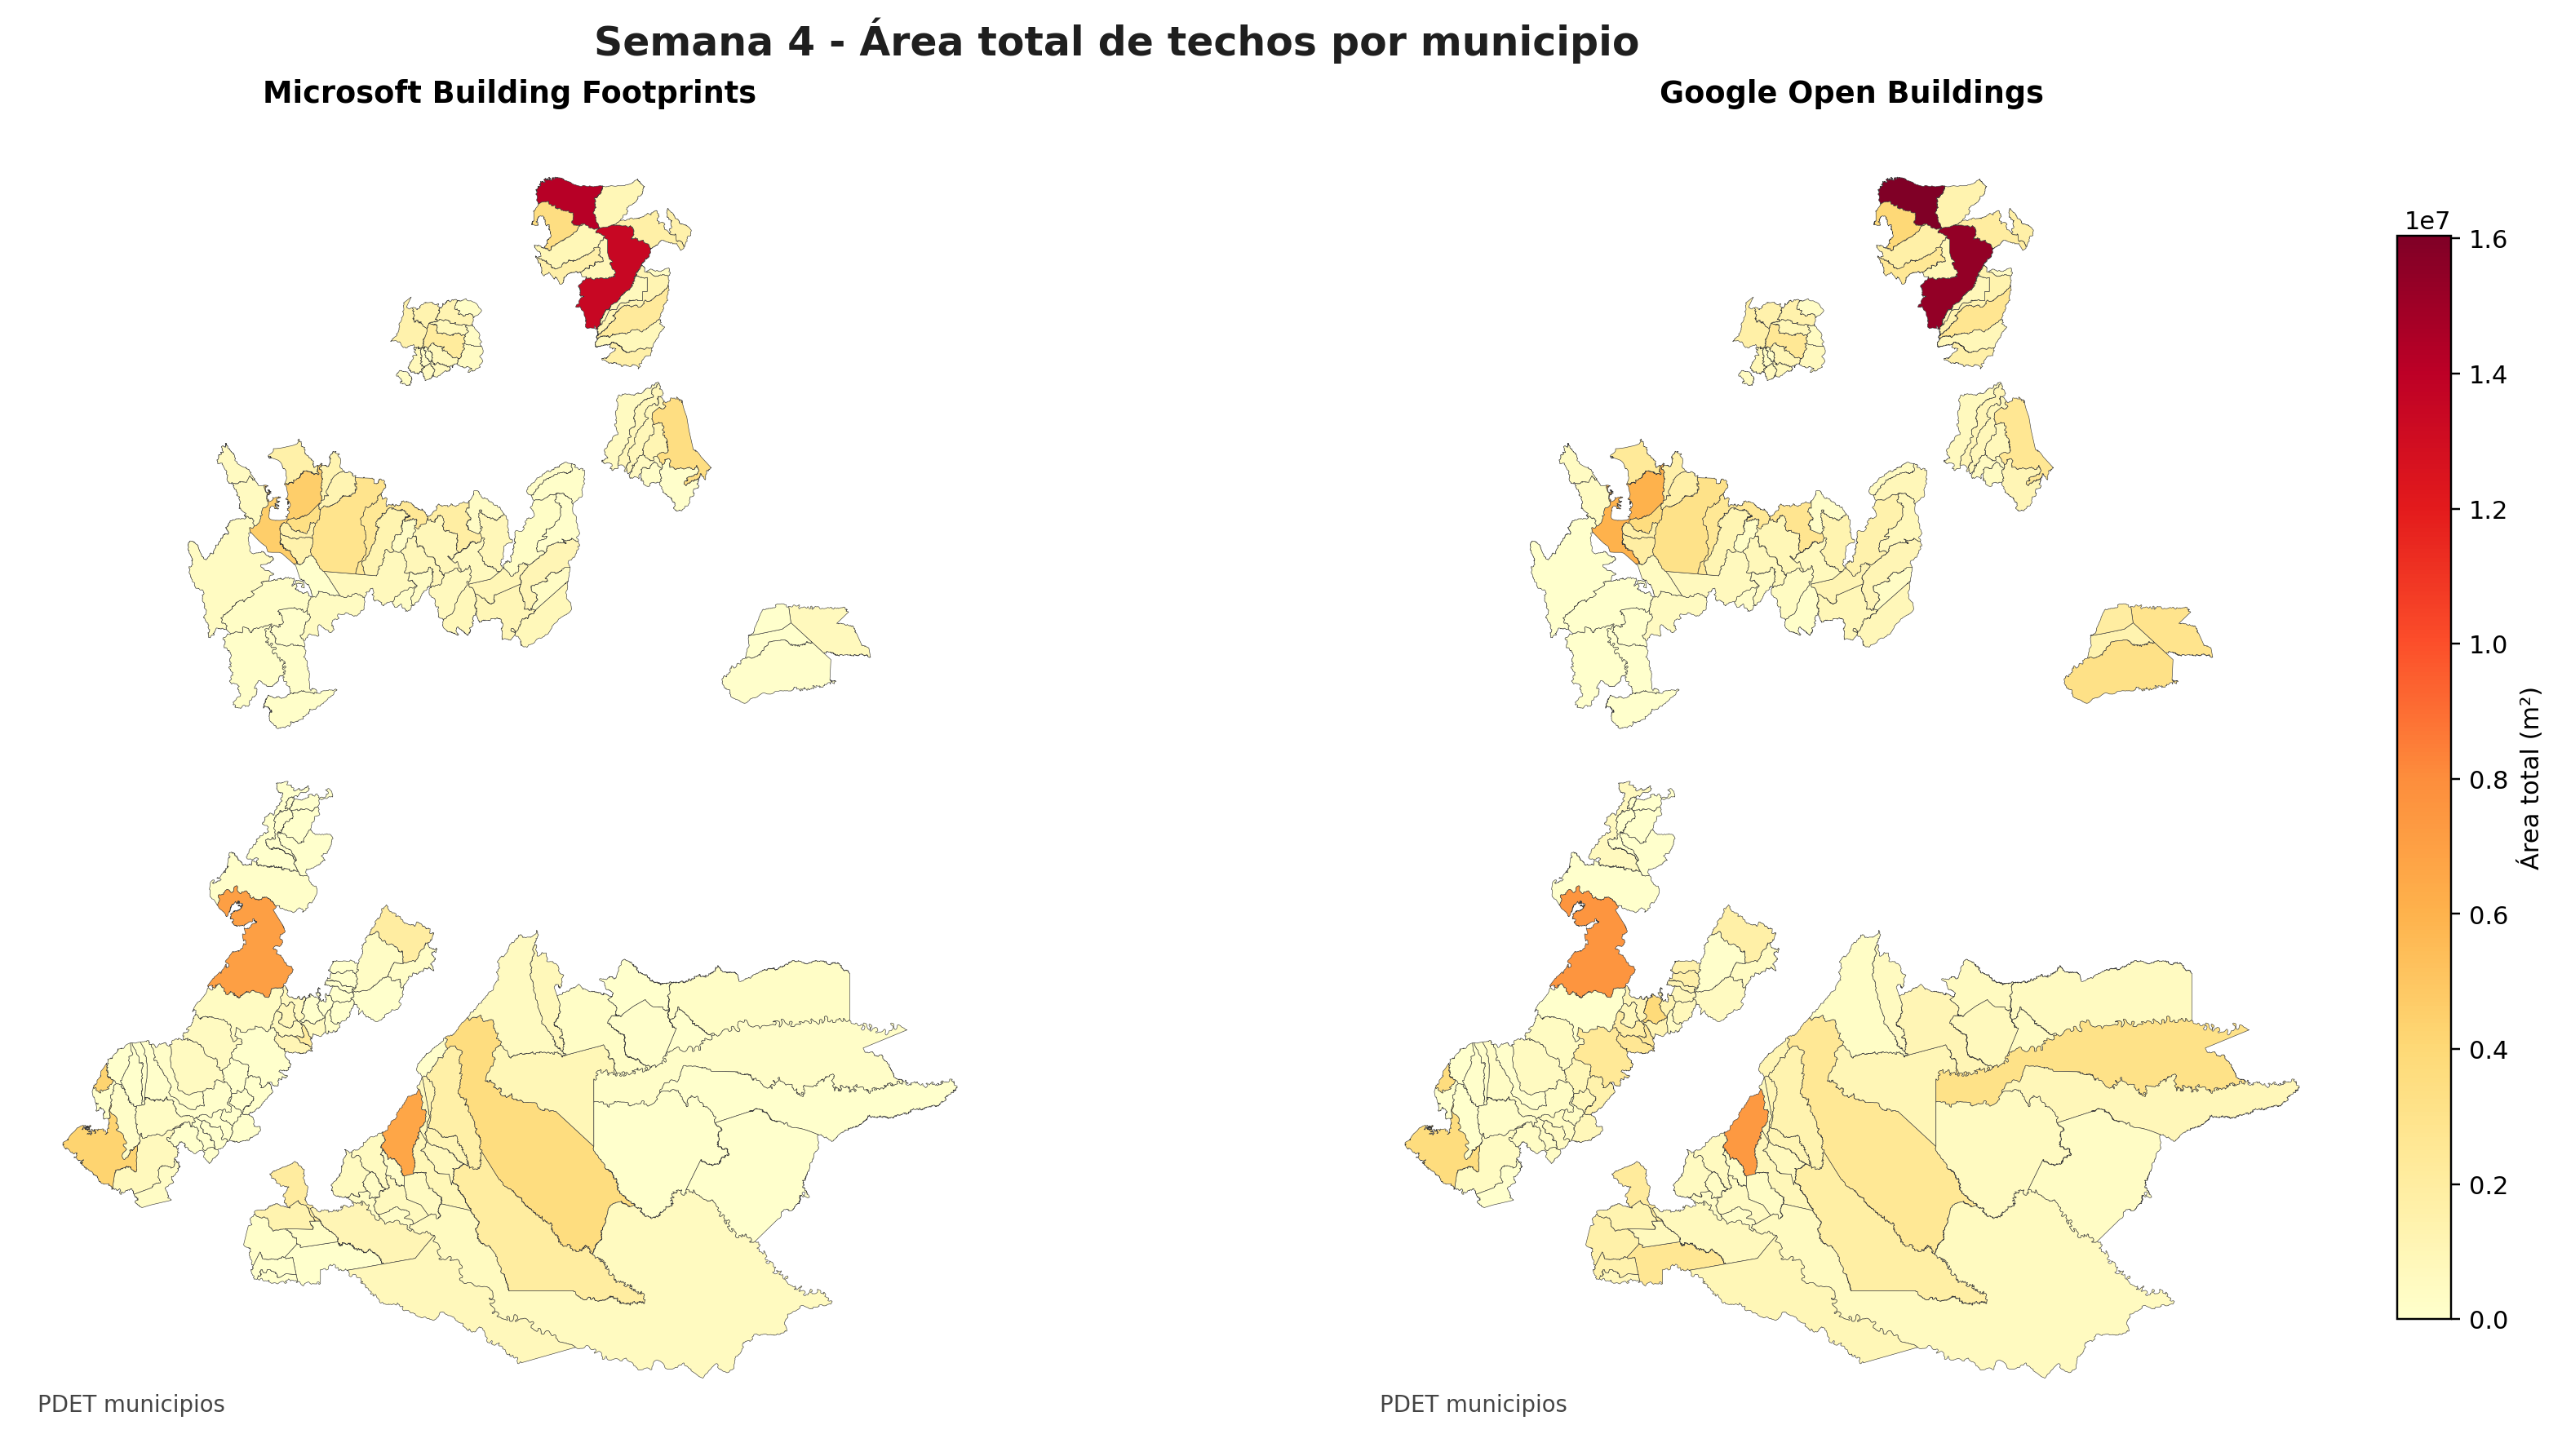
\includegraphics[width=0.98\linewidth]{../maps/week4_area_maps.png}
  \caption{Mapa comparativo por municipio: \textbf{Área total de techos} (Microsoft vs Google). Archivo generado: \texttt{semana\_4/maps/week4\_area\_maps.png}}
  \label{fig:area_maps}
\end{figure}

\begin{figure}[H]
  \centering
  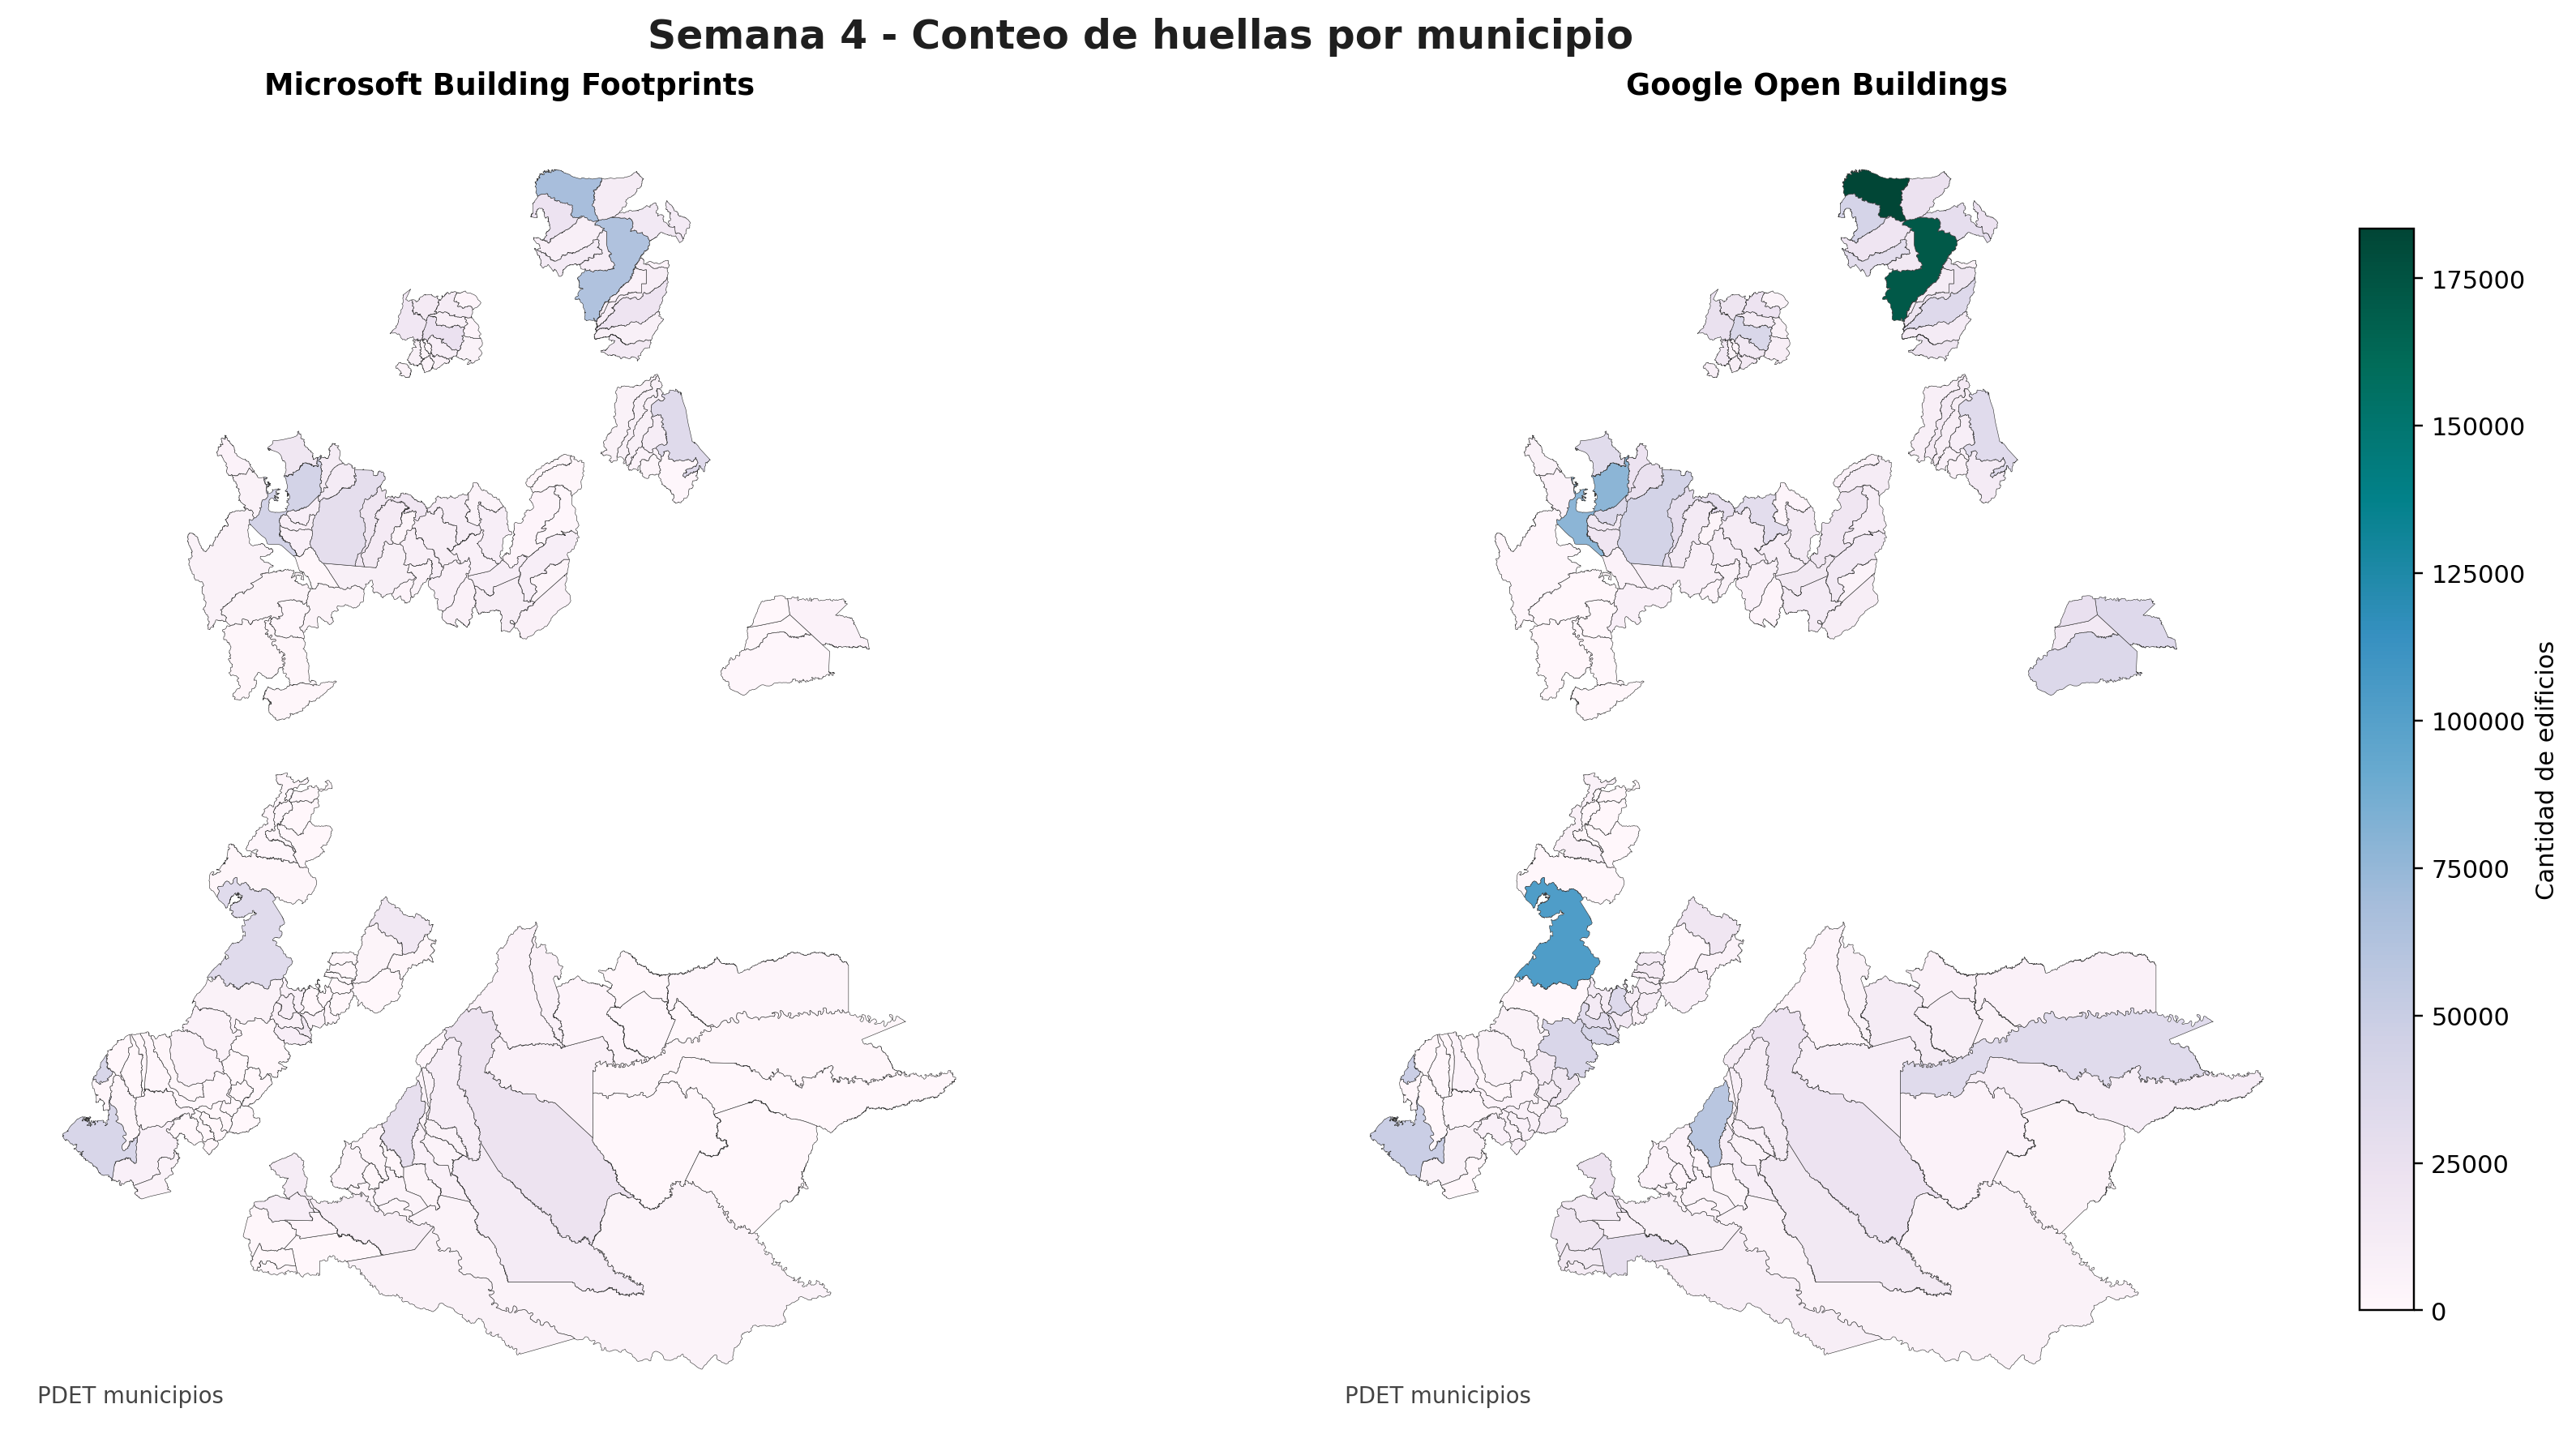
\includegraphics[width=0.98\linewidth]{../maps/week4_count_maps.png}
  \caption{Mapa comparativo por municipio: \textbf{Conteo de huellas} (Microsoft vs Google). Archivo generado: \texttt{semana\_4/maps/week4\_count\_maps.png}}
  \label{fig:count_maps}
\end{figure}

\subsection{Ranking y EDA}

\begin{itemize}
  \item Top 10 calculado por \'area total de techos en ambos datasets.
  \item \texttt{buildings\_microsoft}: 1,237,245 documentos.
  \item \texttt{buildings\_google}: 2,693,803 documentos.
  \item En Google, 100\% de los registros tienen campo de confianza disponible.
  \item Ambos datasets tienen \'indice \texttt{2dsphere}.
\end{itemize}

\section{Evidencia de consola}

\begin{lstlisting}[style=evidence]
============================================================
VERIFICACION DE ARCHIVOS
============================================================

1. Verificando MunicipiosPDET.xlsx...
   MunicipiosPDET.xlsx encontrado

2. Verificando shapefile...
   Shapefile encontrado en MGN_2025_COLOMBIA/ADMINISTRATIVO/MGN_ADM_MPIO_GRAFICO.shp


============================================================
MENU PRINCIPAL
============================================================
1. Cargar municipios PDET en MongoDB
2. Verificar municipios PDET
3. Ingestar huellas de edificios - MICROSOFT
4. Ingestar huellas de edificios - GOOGLE
5. Reparar y reindexar colecciones de edificios
6. Análisis geoespacial (conteo y área por municipio)
7. EDA - Auditoría exploratoria completa

8. Salir

Selecciona una opcion (1-8): 1
============================================================
CONFIGURACION DE MONGODB
============================================================

Ingresa la IP de MongoDB (deja en blanco para localhost): 
Usando MongoDB local: mongodb://localhost:27017/

============================================================
OPCIONES DE CARGA DE DATOS
============================================================

Deseas cargar los datos en MongoDB? (s/n): s
============================================================
INICIANDO CARGA DE MUNICIPIOS PDET EN MONGODB
============================================================

Cargando lista PDET desde Excel...
  Municipios PDET en Excel: 170

Leyendo shapefile...
  Total municipios MGN : 1122
  CRS original         : EPSG:4326
  Municipios PDET encontrados en shapefile: 170
Calculando áreas en EPSG:9377 (Magnus)...

Cargando 170 documentos en MongoDB...
 170 municipios sincronizados
 Índice 2dsphere creado

Verificación
  Documentos en colección : 170
  Índices                 : ['_id_', 'geometry_2dsphere']
  Muestra                 : {'dane_code': '05031', 'area_m2': 1208346188.1, 'name': 'AMALFI'}

Ingesta completada.

============================================================
MENU PRINCIPAL
============================================================
1. Cargar municipios PDET en MongoDB
2. Verificar municipios PDET
3. Ingestar huellas de edificios - MICROSOFT
4. Ingestar huellas de edificios - GOOGLE
5. Reparar y reindexar colecciones de edificios
6. Análisis geoespacial (conteo y área por municipio)
7. EDA - Auditoría exploratoria completa

8. Salir

Selecciona una opcion (1-8): 2
============================================================
CONFIGURACION DE MONGODB
============================================================

Ingresa la IP de MongoDB (deja en blanco para localhost): 
Usando MongoDB local: mongodb://localhost:27017/


============================================================
VERIFICACION DE MUNICIPIOS PDET
============================================================

1. Cargando lista PDET desde Excel...
  Municipios PDET en Excel: 170
   Total municipios PDET esperados: 170

2. Verificando en MongoDB...
   Total municipios PDET en MongoDB: 170

3. Comparando codigos...
   Verificacion exitosa: todos los 170 municipios PDET estan en MongoDB


============================================================
MENU PRINCIPAL
============================================================
1. Cargar municipios PDET en MongoDB
2. Verificar municipios PDET
3. Ingestar huellas de edificios - MICROSOFT
4. Ingestar huellas de edificios - GOOGLE
5. Reparar y reindexar colecciones de edificios
6. Análisis geoespacial (conteo y área por municipio)
7. EDA - Auditoría exploratoria completa

8. Salir

Selecciona una opcion (1-8): 3

-> Verificando dataset Microsoft Buildings en 'ms_buildings/'
  136 particiones ya descargadas en 'ms_buildings/'.
============================================================
CONFIGURACION DE MONGODB
============================================================

Ingresa la IP de MongoDB (deja en blanco para localhost): 
Usando MongoDB local: mongodb://localhost:27017/

============================================================
OPCIONES DE CARGA DE DATOS
============================================================

Deseas cargar los datos en MongoDB? (s/n): s

Cargando datos de MICROSOFT...
  Filtro PDET: 170 municipios cargados
  PDET bbox: (-79.01021097538057, -0.7058400442509765, -69.99510700215114, 11.348889869055824)
  136 particiones totales -- 136 ya cargadas, 0 pendientes.
  Prefiltro por bounding box...
  0 particiones relevantes a procesar.


Creando indice 2dsphere...
-> Asegurando indice 2dsphere en 'buildings_microsoft'...
   Indexacion exitosa en 'buildings_microsoft'


  Ingesta completada: 0 documentos insertados en esta sesion.


============================================================
MENU PRINCIPAL
============================================================
1. Cargar municipios PDET en MongoDB
2. Verificar municipios PDET
3. Ingestar huellas de edificios - MICROSOFT
4. Ingestar huellas de edificios - GOOGLE
5. Reparar y reindexar colecciones de edificios
6. Análisis geoespacial (conteo y área por municipio)
7. EDA - Auditoría exploratoria completa

8. Salir

Selecciona una opcion (1-8): 4

-> Verificando dataset Google Open Buildings en 'google_buildings/'
  20 tiles ya descargados en 'google_buildings/'.
============================================================
CONFIGURACION DE MONGODB
============================================================

Ingresa la IP de MongoDB (deja en blanco para localhost): 
Usando MongoDB local: mongodb://localhost:27017/

============================================================
OPCIONES DE CARGA DE DATOS
============================================================

Deseas cargar los datos en MongoDB? (s/n): s

Cargando datos de GOOGLE...
  Filtro PDET: 170 municipios cargados
  PDET bbox: (-79.01021097538057, -0.7058400442509765, -69.99510700215114, 11.348889869055824)
  20 tiles totales -- 20 ya cargados, 0 pendientes.


Creando indice 2dsphere...
-> Asegurando indice 2dsphere en 'buildings_google'...
   Indexacion exitosa en 'buildings_google'


  Ingesta completada: 0 documentos insertados en esta sesion.


============================================================
MENU PRINCIPAL
============================================================
1. Cargar municipios PDET en MongoDB
2. Verificar municipios PDET
3. Ingestar huellas de edificios - MICROSOFT
4. Ingestar huellas de edificios - GOOGLE
5. Reparar y reindexar colecciones de edificios
6. Análisis geoespacial (conteo y área por municipio)
7. EDA - Auditoría exploratoria completa

8. Salir

Selecciona una opcion (1-8): 6
============================================================
CONFIGURACION DE MONGODB
============================================================

Ingresa la IP de MongoDB (deja en blanco para localhost): 
Usando MongoDB local: mongodb://localhost:27017/


============================================================
 SEMANA 4 - ANALISIS GEOESPACIAL POR MUNICIPIO
 Base de datos: upme-project
============================================================

============================================================
 7. ANALISIS GEOESPACIAL Y AGREGACIONES
============================================================

  Procesando dataset: MICROSOFT
    170/170 ya calculados, 0 pendientes.
    Municipios procesados : 170
    Edificios totales     : 1,235,576
    Area total acumulada  : 159,880,080.08 m2

  Procesando dataset: GOOGLE
    170/170 ya calculados, 0 pendientes.
    Municipios procesados : 170
    Edificios totales     : 2,690,174
    Area total acumulada  : 222,643,644.57 m2

  Resultados almacenados en 'analysis_results'.

============================================================
 8. TOP 10 MUNICIPIOS POR AREA DE TECHOS
============================================================

  ------------------------------------------------------
  Dataset: MICROSOFT
  ------------------------------------------------------
    #    Municipio                 Depto                 Edif.  Area total m2 Area prom m2
    -------------------------------------------------------------------------------------
    1    SANTA MARTA               MAGDALENA            67,615  14,217,875.29       210.28
    2    VALLEDUPAR                CESAR                63,696  13,529,663.43       212.41
    3    BUENAVENTURA              VALLE DEL CAUCA      32,808   7,038,050.92       214.52
    4    FLORENCIA                 CAQUETÁ              26,886   6,680,084.26       248.46
    5    TURBO                     ANTIOQUIA            43,166   4,627,313.82       107.20
    6    SAN ANDRÉS DE TUMACO      NARIÑO               40,025   4,295,233.07       107.31
    7    SAN VICENTE DEL CAGUÁN    CAQUETÁ              22,463   3,629,270.23       161.57
    8    CIÉNAGA                   MAGDALENA            21,915   3,468,723.62       158.28
    9    TIBÚ                      NORTE DE SANTANDER   34,361   3,462,308.40       100.76
    10   APARTADÓ                  ANTIOQUIA             9,806   3,351,302.69       341.76

  ------------------------------------------------------
  Dataset: GOOGLE
  ------------------------------------------------------
    #    Municipio                 Depto                 Edif.  Area total m2 Area prom m2
    -------------------------------------------------------------------------------------
    1    SANTA MARTA               MAGDALENA           183,504  16,036,668.47        87.39
    2    VALLEDUPAR                CESAR               171,414  15,391,687.39        89.79
    3    BUENAVENTURA              VALLE DEL CAUCA     103,109   7,613,831.10        73.84
    4    FLORENCIA                 CAQUETÁ              58,134   7,363,259.52       126.66
    5    TURBO                     ANTIOQUIA            78,526   6,019,578.12        76.66
    6    CIÉNAGA                   MAGDALENA            41,825   3,956,585.22        94.60
    7    SANTANDER DE QUILICHAO    CAUCA                35,681   3,850,787.00       107.92
    8    SAN ANDRÉS DE TUMACO      NARIÑO               49,219   3,665,967.92        74.48
    9    APARTADÓ                  ANTIOQUIA            36,333   3,606,269.94        99.26
    10   TAME                      ARAUCA               35,952   3,200,043.97        89.01

      Mapas generados:
    - semana_4\maps\week4_area_maps.png
    - semana_4\maps\week4_count_maps.png

============================================================
 Analisis geoespacial completado.
============================================================


============================================================
MENU PRINCIPAL
============================================================
1. Cargar municipios PDET en MongoDB
2. Verificar municipios PDET
3. Ingestar huellas de edificios - MICROSOFT
4. Ingestar huellas de edificios - GOOGLE
5. Reparar y reindexar colecciones de edificios
6. Análisis geoespacial (conteo y área por municipio)
7. EDA - Auditoría exploratoria completa

8. Salir

Selecciona una opcion (1-8): 7
============================================================
CONFIGURACION DE MONGODB
============================================================

Ingresa la IP de MongoDB (deja en blanco para localhost): 
Usando MongoDB local: mongodb://localhost:27017/


============================================================
 EDA - BUILDING FOOTPRINTS (Microsoft & Google)
 Base de datos: upme-project
============================================================

============================================================
 1. CONTEO DE DOCUMENTOS POR DATASET
============================================================
  buildings_microsoft    :    1,237,245 documentos  [OK]
  buildings_google       :    2,693,803 documentos  [OK]

============================================================
 2. ESTADISTICAS DE AREA (area_m2 en m2)
============================================================

  ------------------------------------------------------
  Dataset: MICROSOFT
  ------------------------------------------------------
    Conteo          :    1,237,245
    Area total      :  160,168,258.75 m2
    Media           :       129.46 m2
    Desv. estandar  :       250.51 m2
    Minimo          :         9.69 m2
    Maximo          :    44,720.44 m2

    Distribucion por quintil:
    Rango (m2)                              Conteo
    [      9.69 -      39.76]      247,544
    [     39.76 -      63.19]      247,503
    [     63.19 -      94.05]      247,492
    [     94.05 -     154.02]      247,453
    [    154.02 -   44720.44]      247,253

  ------------------------------------------------------
  Dataset: GOOGLE
  ------------------------------------------------------
    Conteo          :    2,693,803
    Area total      :  222,995,983.84 m2
    Media           :        82.78 m2
    Desv. estandar  :       126.40 m2
    Minimo          :         2.51 m2
    Maximo          :    20,916.70 m2

    Distribucion por quintil:
    Rango (m2)                              Conteo
    [      2.51 -      25.94]      538,783
    [     25.94 -      46.20]      538,892
    [     46.20 -      72.11]      538,818
    [     72.11 -     113.88]      538,839
    [    113.88 -   20916.70]      538,471

============================================================
 3. CALIDAD DE DATOS
============================================================

  ------------------------------------------------------
  Dataset: MICROSOFT
  ------------------------------------------------------
    Problema                              Conteo   % del total
    ---------------------------------------------------------
    area_m2 nula                               0        0.00%
    area_m2 <= 0                               0        0.00%
    geometry ausente                           0        0.00%
    sin source                                 0        0.00%

  ------------------------------------------------------
  Dataset: GOOGLE
  ------------------------------------------------------
    Problema                              Conteo   % del total
    ---------------------------------------------------------
    area_m2 nula                               0        0.00%
    area_m2 <= 0                               0        0.00%
    geometry ausente                           0        0.00%
    sin source                                 0        0.00%

============================================================
 4. CONFIDENCE SCORE - Google Open Buildings
============================================================
  Registros con confidence_score:  2,693,803  (100.00%)
  Registros sin confidence_score:          0  (0.00%)

  Media  : 0.7797
  Minimo : 0.6500
  Maximo : 0.9834

  Rango               Conteo          %
  -------------------------------------
  < 0.60                   0      0.00%
  0.60-0.70          431,067     16.00%
  0.70-0.80        1,146,368     42.56%
  0.80-0.90        1,039,868     38.60%
  >= 0.90             76,500      2.84%

============================================================
 5. INDICES EN MONGODB
============================================================

  buildings_microsoft:
    - _id_                            key: {'_id': 1}
    - geometry_2dsphere               key: {'geometry': '2dsphere'}

  buildings_google:
    - _id_                            key: {'_id': 1}
    - geometry_2dsphere               key: {'geometry': '2dsphere'}

============================================================
 6. MUESTRA DE DOCUMENTOS
============================================================

  ------------------------------------------------------
  Dataset: MICROSOFT
  ------------------------------------------------------
{
    "area_m2": 44.39,
    "source": "microsoft",
    "ingested_at": "2026-05-25 03:54:50.354000"
}

  ------------------------------------------------------
  Dataset: GOOGLE
  ------------------------------------------------------
{
    "area_m2": 43.76,
    "source": "google",
    "ingested_at": "2026-05-25 04:22:28.734000",
    "confidence_score": 0.8335
}

============================================================
 7. ANALISIS GEOESPACIAL Y AGREGACIONES
============================================================

  Procesando dataset: MICROSOFT
    170/170 ya calculados, 0 pendientes.
    Municipios procesados : 170
    Edificios totales     : 1,235,576
    Area total acumulada  : 159,880,080.08 m2

  Procesando dataset: GOOGLE
    170/170 ya calculados, 0 pendientes.
    Municipios procesados : 170
    Edificios totales     : 2,690,174
    Area total acumulada  : 222,643,644.57 m2

  Resultados almacenados en 'analysis_results'.

============================================================
 8. TOP 10 MUNICIPIOS POR AREA DE TECHOS
============================================================

  ------------------------------------------------------
  Dataset: MICROSOFT
  ------------------------------------------------------
    #    Municipio                 Depto                 Edif.  Area total m2 Area prom m2
    -------------------------------------------------------------------------------------
    1    SANTA MARTA               MAGDALENA            67,615  14,217,875.29       210.28
    2    VALLEDUPAR                CESAR                63,696  13,529,663.43       212.41
    3    BUENAVENTURA              VALLE DEL CAUCA      32,808   7,038,050.92       214.52
    4    FLORENCIA                 CAQUETÁ              26,886   6,680,084.26       248.46
    5    TURBO                     ANTIOQUIA            43,166   4,627,313.82       107.20
    6    SAN ANDRÉS DE TUMACO      NARIÑO               40,025   4,295,233.07       107.31
    7    SAN VICENTE DEL CAGUÁN    CAQUETÁ              22,463   3,629,270.23       161.57
    8    CIÉNAGA                   MAGDALENA            21,915   3,468,723.62       158.28
    9    TIBÚ                      NORTE DE SANTANDER   34,361   3,462,308.40       100.76
    10   APARTADÓ                  ANTIOQUIA             9,806   3,351,302.69       341.76

  ------------------------------------------------------
  Dataset: GOOGLE
  ------------------------------------------------------
    #    Municipio                 Depto                 Edif.  Area total m2 Area prom m2
    -------------------------------------------------------------------------------------
    1    SANTA MARTA               MAGDALENA           183,504  16,036,668.47        87.39
    2    VALLEDUPAR                CESAR               171,414  15,391,687.39        89.79
    3    BUENAVENTURA              VALLE DEL CAUCA     103,109   7,613,831.10        73.84
    4    FLORENCIA                 CAQUETÁ              58,134   7,363,259.52       126.66
    5    TURBO                     ANTIOQUIA            78,526   6,019,578.12        76.66
    6    CIÉNAGA                   MAGDALENA            41,825   3,956,585.22        94.60
    7    SANTANDER DE QUILICHAO    CAUCA                35,681   3,850,787.00       107.92
    8    SAN ANDRÉS DE TUMACO      NARIÑO               49,219   3,665,967.92        74.48
    9    APARTADÓ                  ANTIOQUIA            36,333   3,606,269.94        99.26
    10   TAME                      ARAUCA               35,952   3,200,043.97        89.01

============================================================
 9. TABLA COMPARATIVA MICROSOFT vs GOOGLE
============================================================
  Metrica                              Microsoft          Google
  --------------------------------------------------------------
  Total documentos                     1,237,245       2,693,803
  Area media (m2)                         129.46           82.78
  Area minima (m2)                          9.69            2.51
  Area maxima (m2)                     44,720.44       20,916.70
  Desv. estandar (m2)                     250.51          126.40
  Area total acumulada (m2)          160,168,259     222,995,984
  Indice 2dsphere                             Si              Si

============================================================
 EDA completado.
============================================================
\end{lstlisting}

\section{Interpretaci\'on t\'ecnica}

Los datos observados confirman que la decisi\'on de usar MongoDB con soporte espacial fue correcta para este caso. El n\'umero de edificios procesados es alto, pero la combinaci\'on de \texttt{STRtree}, prefiltrado por \textit{bounding box}, procesamiento por chunks e \'indices \texttt{2dsphere} permite ejecutar el flujo sin depender de herramientas GIS externas para el cruce principal.

Adem\'as, el dise\~no del c\'odigo deja dos ventajas claras:

\begin{itemize}
  \item el proceso es incremental y reproducible, porque se guarda el progreso por archivo;
  \item el resultado es auditable, porque la EDA expone conteos, estad\'isticas, calidad y ejemplos de documentos.
\end{itemize}

\section{Conclusi\'on}

La implementaci\'on actual cumple el objetivo de la semana 4: estimar n\'umero y \'area total de techos por municipio PDET a partir de dos fuentes abiertas, almacenar resultados persistentes y dejar un flujo reproducible para defensa t\'ecnica. La documentaci\'on y el c\'odigo est\'an alineados en torno a la misma arquitectura: descarga, verificaci\'on, carga territorial, ingesta de huellas, an\'alisis geoespacial y auditor\'ia final.

\end{document}